%%%%%%%%%%%%%%%%%%%%%%%%%%%%%%%%%%%%%%%%%
% Journal Article
% LaTeX Template
% Version 1.4 (15/5/16)
%
% This template has been downloaded from:
% http://www.LaTeXTemplates.com
%
% Original author:
% Frits Wenneker (http://www.howtotex.com) with extensive modifications by
% Vel (vel@LaTeXTemplates.com)
%
% License:
% CC BY-NC-SA 3.0 (http://creativecommons.org/licenses/by-nc-sa/3.0/)
%
%%%%%%%%%%%%%%%%%%%%%%%%%%%%%%%%%%%%%%%%%

%----------------------------------------------------------------------------------------
%	PACKAGES AND OTHER DOCUMENT CONFIGURATIONS
%----------------------------------------------------------------------------------------

\documentclass[twoside,twocolumn]{article}

\usepackage{blindtext} % Package to generate dummy text throughout this template 

\usepackage[sc]{mathpazo} % Use the Palatino font
\usepackage[T1]{fontenc} % Use 8-bit encoding that has 256 glyphs
\linespread{1.05} % Line spacing - Palatino needs more space between lines
\usepackage{microtype} % Slightly tweak font spacing for aesthetics

\usepackage[english]{babel} % Language hyphenation and typographical rules

\usepackage[hmarginratio=1:1,top=32mm,columnsep=20pt]{geometry} % Document margins
\usepackage[hang, small,labelfont=bf,up,textfont=it,up]{caption} % Custom captions under/above floats in tables or figures
\usepackage{booktabs} % Horizontal rules in tables

\usepackage{lettrine} % The lettrine is the first enlarged letter at the beginning of the text

\usepackage{enumitem} % Customized lists
\setlist[itemize]{noitemsep} % Make itemize lists more compact

\usepackage{abstract} % Allows abstract customization
\renewcommand{\abstractnamefont}{\normalfont\bfseries} % Set the "Abstract" text to bold
\renewcommand{\abstracttextfont}{\normalfont\small\itshape} % Set the abstract itself to small italic text

\usepackage{titlesec} % Allows customization of titles
\renewcommand\thesection{\Roman{section}} % Roman numerals for the sections
\renewcommand\thesubsection{\roman{subsection}} % roman numerals for subsections
\titleformat{\section}[block]{\large\scshape\centering}{\thesection.}{1em}{} % Change the look of the section titles
\titleformat{\subsection}[block]{\large}{\thesubsection.}{1em}{} % Change the look of the section titles
\usepackage{graphicx}
\usepackage{fancyhdr} % Headers and footers
\pagestyle{fancy} % All pages have headers and footers
\fancyhead{} % Blank out the default header
\fancyfoot{} % Blank out the default footer
%\fancyhead[C]{Running title $\bullet$ June 2016 $\bullet$ Vol. XXI, No. 1} % Custom header text
\fancyfoot[RO,LE]{\thepage} % Custom footer text

\usepackage{titling} % Customizing the title section

\usepackage{hyperref} % For hyperlinks in the PDF

%----------------------------------------------------------------------------------------
%	TITLE SECTION
%----------------------------------------------------------------------------------------

\setlength{\droptitle}{-4\baselineskip} % Move the title up

\pretitle{\begin{center}\Huge\bfseries} % Article title formatting
\posttitle{\end{center}} % Article title closing formatting
\title{Virality of Internet Articles} % Article title
\author{%
\textsc{Uwe-Herbert Hoenig} \\[1ex] % Your name
\normalsize Barcelona Graduate School of Economics \\ % Your institution
\normalsize \href{mailto:uweherbert.honig@barcelonagse.eu}{uweherbert.honig@barcelonagse.eu} % Your email address
%\and % Uncomment if 2 authors are required, duplicate these 4 lines if more
%\textsc{Jane Smith}\thanks{Corresponding author} \\[1ex] % Second author's name
%\normalsize University of Utah \\ % Second author's institution
%\normalsize \href{mailto:jane@smith.com}{jane@smith.com} % Second author's email address
}
%\today
\date{27 June 2016} % Leave empty to omit a date
\renewcommand{\maketitlehookd}{%
\begin{abstract}
\noindent 
What is read and what is shared is often different.  What is it about a piece of content - an article, a picture, a video that took it from simply interesting to interesting and shareable? What pushes someone to not only read a story but to pass it on? In this project I take a technical approach to understand virality through text mining methods. Using internet articles from the famous social media blog Mashable.com over a 1-month period I intend to classify which articles were shared a lot of times (i.e. went viral). I try various classification algorithms of which the best one yields a 54 \% accuracy score, thereby beating the base line of 50\% by a small margin. Furthermore, the analysis indicates positive content to be more viral than negative content. However, the relationship between emotion and social transmission is more complex than valence alone. Virality is partially driven by physiological arousal and the context of the moment it was read. Hence, more investigation is needed.
\end{abstract}
}

%----------------------------------------------------------------------------------------

\begin{document}

% Print the title
\maketitle

%----------------------------------------------------------------------------------------
%	ARTICLE CONTENTS
%----------------------------------------------------------------------------------------

\section{Introduction}

\lettrine[nindent=0em,lines=3]{W} hat makes an article go viral? Authenticity, humor (a picture of a dog on a skateboard) or lastly, controversy and debate (Brexit) - many characteristics may come to mind. However, a writer faces the problem that there is no guaranteed formula of success (yet). In fact, to manufacture or predict whether an article will go viral may depend on the skill of the author, experience and maybe even some luck. Oftentimes, it is just the basics that one would assume that make it share-worthy: insightful and timely articles that tap into some sort of social commentary at that moment. 

\subsection{Historical Analogue}
Interestingly enough, this question predates by centuries. In 350 B.C., Aristotle was already wondering what could make content - in his case, a speech persuasive and memorable enough, so that its ideas would pass from person to person. The answer, he argued, was three principles: ethos, pathos, and logos.\footnote{http://plato.stanford.edu/entries/aristotle-rhetoric/} In his "Modes of Persuasion", content should have an ethical appeal, an emotional appeal, or a logical appeal. A rhetorician strong on all three was likely to leave behind a persuaded audience. Replace rhetorician with online content creator, and Aristotle's insights seem entirely modern. 
%------------------------------------------------

\section{Data}
The data used in this analysis are articles published by Mashable (www.mashable.com), a "leading media site for the Connected Generation and the voice of digital culture" as they claim. The website covers a variety of different topics, however, recently Mashable has moved away from covering world news and politics and towards "core coverage" topics such as technology, web culture, science, social media, entertainment, business and lifestyle.

I have a collection of labeled url links, i.e. links for both viral as well as nonviral articles. The articles were collected during the month of May 2015 and their virality (boolean variable) was labeled according to the number of shares during the given timeframe. Shares is a continuously valued variable that was transformed into a boolean at a certain shares-cutoff. \footnote{Source of Data: Kelwin Fernandes}

Excluding all urls that were not accessible anylonger or simply flawed I have a final corpus consisting of 29875 articles with an average article length of about 300 words.

\subsection{Extracting Content}
My python webscraper script takes in 30 thousand links and checks them for validity using the \emph{try except} syntax. The scraping function has an inbuilt delay to avoid being banned by Mashable's servers and saves the scraped content "on the go" in batches after every 100 iterations. This reduces the risk of loosing all progress of scraping in case of an error.
In the end I store the accepted urls and the extracted content of viral as well as nonviral articles in separate .txt files. Also, I store all rejected urls which in total attributed to only < 0.5\% of all urls.

\begin{table}[!htb]
\caption{Number of Articles}
\centering
\begin{tabular}{llr}
\toprule
\multicolumn{2}{c}{Type} \\
\cmidrule(r){1-2}
viral & nonviral & avg. \# words \\
\midrule
6727 & 23148 & 282 \\
%\bottomrule
\end{tabular}
\end{table}

%------------------------------------------------

\section{Question}
As mentioned in the abstract the goal is to be able to predict whether an article can be classified as viral solely based on its text content. 
Obviously, we have a 50\% chance by simply guessing, however, the goal is to achieve a high score given the insights we may find in the different texts.

\section{Cleaning criteria}
After having saved all documents I use an extensive cleaning script in python that contains the following key cleaning criteria.

\begin{itemize}

\item regular expression 
\item stopwords (english stopwords, punctuation)
\item English words consisting in the english (US) dictionary
\item tokenize (length > 2)
\item lower the words
\item stemming

The biggest problem I faced were scrambled words ( "zzbbeettgg", "mmyyyherie") that may arose during the scraping process. My analysis was majorly affected, so I decided to remove all non-english words altogether. This even had a positive result  on my prediction performance, as I will later discuss. However, the biggest drawback is that all content specific words (Flickr, Kim Kardashian, Elon Musk etc.) are now removed, if they don't happen to be part of the current dictionary.
\end{itemize}

\section{Exploratory Analysis}
As a first step we want to explore the dataset: identify possible mistakes in words and explore possible correlations between features. We see the most frequent viral words depicted in the wordcloud model below. In addition I compute the tdf-idf statistic that is intended to reflect how important a word is to a document in this corpus.
\begin{figure}[!htb]
  \caption{Viral words}
  \centering
    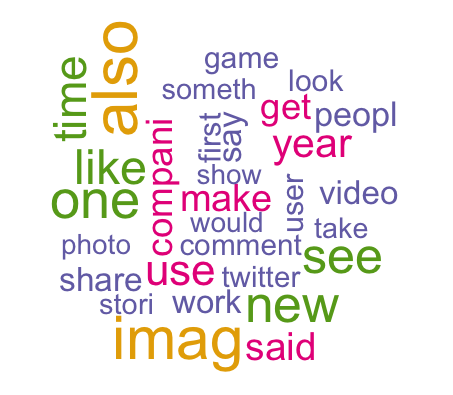
\includegraphics[width=0.4\textwidth]{viral.png}
\end{figure}

\begin{figure}[!htb]
  \caption{Viral words tf-idf}
  \centering
    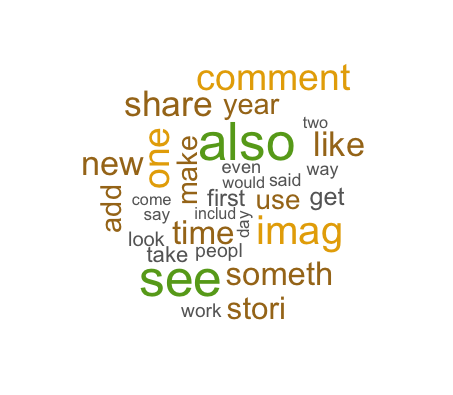
\includegraphics[width=0.5\textwidth]{viral_tfidf.png}
\end{figure}

The results are not too surprising given that articles contain most of these words.
\subsection{Further Analysis}
Furthermore, I used the keywords from the url of each article to explore their correlations with the popularity.
The approach can be summarised in the following steps:

\begin{itemize}

\item First we obtain and store the list of keywords for each class in the training set.
\item From the list of all keywords of the testing set, remove the top 10\% most frequent words.
\item Intersect the test and training lists to obtain the class-wise keywords which potentially have predictive power
\item Remove prepositions, adjectives, verbs, nouns, numbers and other frequently used words.
\item Remove all common keywords across classes in order to obtain a final list of unique keywords per class.
\item Obtain class predictions for the testing set if the url contains keywords belonging to one of the classes
(breaking the ties in favour of higher popularity).
I tested and tuned the above approach taking random splits of the training set and choosing the one that
maximized the number of common words between the out of sample and testing set.

Some interesting results: Here are some of the keywords picked by the algorithm belonging to the classes:
\item Non-viral: systems, navy, spies, cheerleader, supernova, dubai, seahawks, complaints, hotmail
\item Viral: kiss, championships, nasty, changed, heroin
\end{itemize} 

\section{Classification Methods}
We start by establishing a baseline accuracy by using a very simple method. Moving forward, all the more complex methods will be benchmarked against this.

\begin{enumerate}
\item Simple Model (Logistic Regression / Bow)
\item tf-idf
\item SVD, LDA
\item Visualization of Train/Test-Accuracy results
\item Interpretation
\end{enumerate}


\begin{table}[!htb]
\caption{AUC-scores of used methods}
\centering
\begin{tabular}{llr}
\toprule
\multicolumn{2}{c}{Type} \\
\cmidrule(r){1-2}
Train & Test & Algorithm \\
\midrule
56.0\% & 53.7\% & Logistic Reg. on SVD\footnote{110 principal components gave the best result} \\
50.5\% & 52.9 \% & Logistic Reg. on tf-idf\\
61.0\% & 52.2\% & Logistic Reg. on dtm\\
100.0\% & 51.1\% & Random Forest on SVD \\
%\bottomrule
\end{tabular}
\end{table}
My highest score of 53.7\% in testing came from using a Logistic Regression on the SVD transformed tf-idf document term matrix.
As with random forest, overfitting was to be expected. Logisitic regression benefited a bit from performing a singular value decomposition. 
\begin{table}[]
\centering
\caption{Most important features}
\label{my-label}
\begin{tabular}{ccc}
\midrule
june & age & grab   \\
turn & better & attempt   \\
freeman & feed & system   \\
comment & imag & scroll   \\
\bottomrule
\end{tabular}
\end{table}

\subsection{Latent Dirichlet Allocation}
Let us investigate an LDA analysis. I created a function that optimizes for the number of topics chosen in the range of 1 to 20 and it yields a result of 10 topics. I used the labeled documents to build our corpus with probabilities of each article belonging to a set of Topics determined by Latent Dirichlet Allocation. The result was an AUC score of 51.1 \% which is not a huge improvement. 

\subsection{Topic cluster}
\begin{itemize}
\item (0, u'0.012*award + 0.012*star + 0.012*show + 0.011*film')
\item (1, u'0.013*said + 0.009*polic + 0.007*protest + 0.006*peopl')
\item (2, u'0.012*devic + 0.010*appl + 0.010*also + 0.009*new')
\item (3, u'0.009*imag + 0.008*citi + 0.007*photo + 0.007*space')
\item (4, u'0.009*compani + 0.008*servic + 0.008*also + 0.008*said')
\item (5, u'0.018*imag + 0.010*video + 0.010*courtesi + 0.008*also')
\item (6, u'0.010*research + 0.008*studi + 0.007*space + 0.007*univers')
\item (7, u'0.010*use + 0.009*one + 0.009*photo + 0.009*imag')
\item (8, u'0.010*compani + 0.009*twitter + 0.009*social + 0.008*new')
\item (9, u'0.019*game + 0.015*team + 0.015*world + 0.009*player')
\end{itemize}

Each generated topic is separated by a comma. Within each topic are the four most probable words to appear in that topic. The model is reasonable: Topic 1 contains: award, star, show, film - which go well together. LDA assumes documents are produced from a mixture of topics. Those topics then generate words based on their probability distribution.

%------------------------------------------------

\section{Conclusion}
The overall objective was to classify documents according to virality. This has been achieved using standard algorithmic methods as well as some feature engineering. However, more work is needed in order to improve the overall score of prediction.
The irony, of course, is that the more data we mine, and the closer we come to determining a precise calculus of sharing, the less likely it will be for what we know to remain true. If emotion and arousal are key, then, in a social application of the observer effect, we may be changing what will become popular. "What used to be emotionally arousing simply isn't any longer." "If everyone is perfectly implementing the best headline to pass on, it's not as effective any more," (Berger 2016). 
%----------------------------------------------------------------------------------------
%	REFERENCE LIST
%----------------------------------------------------------------------------------------

\begin{thebibliography}{99} % Bibliography - this is intentionally simple in this template

\bibitem{Simon & Schuster}Jonah Berger {\em Contagious: Why Things Catch On}
\bibitem{notes} http://www.newyorker.com/tech/elements/the-six-things-that-make-stories-go-viral-will-amaze-and-maybe-infuriate-you
\end{thebibliography}

%----------------------------------------------------------------------------------------

\end{document}
